\documentclass{beamer}
%kdfj
\usetheme[secheader]{Boadilla}
\setbeamertemplate{footline} {
  %\leavevmode%
  \hbox{%
  \begin{beamercolorbox}[wd=.5\paperwidth,ht=2.25ex,dp=1ex,left]{author in head/foot}%
    \usebeamerfont{author in head/foot}\hspace*{2ex}\insertshortauthor~~(adraeger@cern.ch)
  \end{beamercolorbox}%
  \begin{beamercolorbox}[wd=.5\paperwidth,ht=2.25ex,dp=1ex,right]{date in head/foot}%
    \usebeamerfont{date in head/foot}\insertshorttitle,~
    \insertshortdate{}\hspace*{1em}
    \insertframenumber{} / \inserttotalframenumber\hspace*{2ex}
  \end{beamercolorbox}}%
  \vskip0pt%
}
\beamertemplatenavigationsymbolsempty

\usepackage[percent]{overpic}
\usepackage{tikz}
%\usetikzlibrary{positioning,fit,shapes.arrows,shapes.geometric,shapes.misc,shapes.multipart,calc,shadows}
\tikzstyle{every picture}+=[remember picture]
\usepackage{booktabs}
\usepackage{graphicx}
\usepackage{rotating}
\usepackage{wasysym}
\usepackage{marvosym}
\usepackage{amssymb}
\usepackage{xcolor}
\graphicspath{{../../logo/}{figures/}{../../graphic-common/}}

\input{definitions.tex}
\newcommand{\lib}[1]{\tiny #1}

% Title etc
\vskip2cm
\title[RA2/b Meeting]{Classical Lost-Lepton Background}
\subtitle{Study of Lepton:\\Mini Isolation vs Classical Isolation\\ Lost-Lepton Method with Isolated Track Veto\\ Exlusive Search Bin Definition}
\author[Arne-Rasmus~Dr\"ager]{
  Arne-Rasmus~Dr\"ager(Uni Hamburg)
}
\date[March 17, 2015]{March 17, 2015
  \vskip1cm
  \begin{center}
    \includegraphics[height=1.5cm]{Universitaet-Hamburg-Logo.jpg}
    \hskip8cm
    \includegraphics[height=1.5cm]{CMSlogo.jpeg}
  \end{center}
}

% pdflatex packages
\hypersetup{bookmarks=true}
\hypersetup{unicode=false}
\hypersetup{pdftitle={Lost-Lepton}}
\hypersetup{pdfauthor={Arne-Rasmus~Dr\"ager}}


\begin{document}
% ==================================================
% --------------------------------------------------
\begin{frame}
  \titlepage
\end{frame}
\section{Lost-Lepton Method}
\begin{frame}
 \begin{block}{}
 \centering
 \Large Mini-Isolation \& Lost-Lepton Method
 \end{block}
\end{frame}
\subsection{Lost-Lepton Method}
\begin{frame}
 \begin{center}
\begin{tikzpicture}
    \node[anchor=south west,inner sep=0] (image) at (0,0) {\includegraphics[width=0.75\textwidth]{figures/Sketches/LostLeptonSketch_mu_pred_full.pdf}};
    \begin{scope}[x={(image.south east)},y={(image.north west)}]
%         \draw[red,ultra thick,rounded corners] (0.62,0.65) rectangle (0.78,0.75);
        \draw[red,ultra thick,rounded corners] (0.60,0.01) rectangle (0.75,0.99); % cordinates unten links(x,y) oben rechts(x,y)
    \end{scope}
\end{tikzpicture}

 \end{center}
 \begin{itemize}
  \item Focus on the isolation definition and the estimation of the lost-leptons due to failing isolation
 \end{itemize}
\end{frame}


\section{Mini Isolation VS Classical Isolation}
\subsection{Mini Isolation (UCSB approach \href{https://indico.cern.ch/event/368826/contribution/3/material/slides/0.pdf}{Adam talk}) vs Classical Isolation}
\begin{frame}
%  \frametitle{Mini Isolation (UCSB approach \href{https://indico.cern.ch/event/368826/contribution/3/material/slides/0.pdf}{Adam talk}) vs Classical Isolation}
  \begin{columns}
   \begin{column}{0.65\textwidth}
   Mini Isolation (reminder):
 \begin{itemize}
  \item Variable isolation cone $R$ depending on lepton \pt   
  \item Current used $\Delta R$:
  \begin{itemize}
   \item Max isolation cone $R = 0.2$ ($\pt,lep \leq50 GeV$)
   \item Med isolation cone $R=\frac{10 GeV}{\pt,lep}$ ($50 GeV \geq\pt,lep \leq200 GeV$)
   \item Min isolation cone $R = 0.05$ ($\pt,lep \geq200 GeV$)
  \end{itemize}
 \end{itemize}
 \end{column}
 \begin{column}{0.35\textwidth}
 \vskip3cm
  \begin{overpic}[width=1.0\textwidth]{figures/Sketches/miniIso.png}
%  \put(0,10){\rotatebox{-0}{\normalsize Expectation \& Prediction using single $\mu$ control sample (CS)}}
 \end{overpic}
 \end{column}
 \end{columns}
 
  \begin{center}
  \begin{tabular}{|l||c|c|}
  \hline
     & Classical RA2b & Mini isolation\\ \hline
Isolation radius: e & $\Delta R < 0.3$  & $0.05<\Delta R<0.2$  \\ \hline
Isolation radius: $\mu$ & $\Delta R < 0.4$  & $0.05<\Delta R<0.2$  \\ \hline
Rel isolation cut: e & $\delta \beta I(rel)<0.16/0.21$ &  $\delta \beta I(rel)<0.4 (0.2)$ \\ \hline
Rel isolation cut: $\mu$ & $\delta \beta I(rel)<0.2$ &  $\delta \beta I(rel)<0.1 (0.2)$ \\ \hline
  \end{tabular}
  \end{center}
\end{frame}
\subsection{Talk Overview}

\begin{frame}
\frametitle{This Talk:}
\begin{itemize}
 \item Investigate 3 isolation definitions
 \item Compare isolation efficiencies (over all \& dependency on variables)
 \item Check purity of single lep control-sample (CS)
 \item Study closure test
\end{itemize}
\vskip1cm
 \begin{columns}

   \begin{column}{0.33\textwidth}
   \begin{itemize}
    \item Classical RA2b isolation
    \end{itemize}
   $e : \delta \beta I(rel)<0.16/0.21$
   $\mu : \delta \beta I(rel)<0.2$
 \end{column}
 \begin{column}{0.33\textwidth}
  \begin{itemize}
   \item MiniIsolation 1 (Jack):
   \end{itemize}
   $e : \delta \beta I(rel)<0.1$
   $\mu : \delta \beta I(rel)<0.4$
   
 \end{column}
 \begin{column}{0.33\textwidth}
  \begin{itemize}
   \item MiniIsolation 2:
   \end{itemize}
   $e : \delta \beta I(rel)<0.1$
   $\mu : \delta \beta I(rel)<0.2$
 
 \end{column}
 \end{columns}
\end{frame}

\subsection{Comparison efficiencies $\mu$}
\begin{frame}
  \begin{columns}

   \begin{column}{0.33\textwidth}
   \begin{itemize}
    \item Classical RA2b isolation
    \end{itemize}
    \small
   $\mu : \delta \beta I(rel)<0.2$
   \begin{tikzpicture}
    \node[anchor=south west,inner sep=0] (image) at (0,0) {\includegraphics[width=1.\textwidth]{figures/ra2classic/MuIsoHT1D.pdf}};
    \begin{scope}[x={(image.south east)},y={(image.north west)}]
%         \draw[red,ultra thick,rounded corners] (0.62,0.65) rectangle (0.78,0.75);
%         \draw[red,ultra thick,rounded corners] (0.60,0.01) rectangle (0.75,0.99); % cordinates unten links(x,y) oben rechts(x,y)
    \end{scope}
\end{tikzpicture}
   \begin{tikzpicture}
    \node[anchor=south west,inner sep=0] (image) at (0,0) {\includegraphics[width=1.\textwidth]{figures/ra2classic/MuPurityMHT1D.pdf}};
    \begin{scope}[x={(image.south east)},y={(image.north west)}]
%         \draw[red,ultra thick,rounded corners] (0.62,0.65) rectangle (0.78,0.75);
%         \draw[red,ultra thick,rounded corners] (0.60,0.01) rectangle (0.75,0.99); % cordinates unten links(x,y) oben rechts(x,y)
    \end{scope}
\end{tikzpicture}
\begin{itemize}
 \item Eff: 83\% Purity: 99\%\\
 \ttbar \wpj (qcd 0\%)
\end{itemize}

 \end{column}
 \begin{column}{0.33\textwidth}
  \begin{itemize}
   \item MiniIsolation 1 (Jack):
   \end{itemize}
    \small
   $\mu : \delta \beta I(rel)<0.4$
   \begin{tikzpicture}
    \node[anchor=south west,inner sep=0] (image) at (0,0) {\includegraphics[width=1.\textwidth]{figures/miniIsoJack/MuIsoHT1D.pdf}};
    \begin{scope}[x={(image.south east)},y={(image.north west)}]
%         \draw[red,ultra thick,rounded corners] (0.62,0.65) rectangle (0.78,0.75);
%         \draw[red,ultra thick,rounded corners] (0.60,0.01) rectangle (0.75,0.99); % cordinates unten links(x,y) oben rechts(x,y)
    \end{scope}
\end{tikzpicture}
   \begin{tikzpicture}
    \node[anchor=south west,inner sep=0] (image) at (0,0) {\includegraphics[width=1.\textwidth]{figures/miniIsoJack/MuPurityMHT1D.pdf}};
    \begin{scope}[x={(image.south east)},y={(image.north west)}]
%         \draw[red,ultra thick,rounded corners] (0.62,0.65) rectangle (0.78,0.75);
%         \draw[red,ultra thick,rounded corners] (0.60,0.01) rectangle (0.75,0.99); % cordinates unten links(x,y) oben rechts(x,y)
    \end{scope}
\end{tikzpicture}
   \begin{itemize}
 \item Eff: 97\% Purity: 97\%\\
 \ttbar \wpj (qcd 0\%)
\end{itemize}
 \end{column}
 \begin{column}{0.33\textwidth}
  \begin{itemize}
   \item MiniIsolation 2:
   \vskip0.5cm
   \end{itemize}
    \small
   $\mu : \delta \beta I(rel)<0.2$
   \begin{tikzpicture}
    \node[anchor=south west,inner sep=0] (image) at (0,0) {\includegraphics[width=1.\textwidth]{figures/miniIsoStandard/MuIsoHT1D.pdf}};
    \begin{scope}[x={(image.south east)},y={(image.north west)}]
%         \draw[red,ultra thick,rounded corners] (0.62,0.65) rectangle (0.78,0.75);
%         \draw[red,ultra thick,rounded corners] (0.60,0.01) rectangle (0.75,0.99); % cordinates unten links(x,y) oben rechts(x,y)
    \end{scope}
\end{tikzpicture}
   \begin{tikzpicture}
    \node[anchor=south west,inner sep=0] (image) at (0,0) {\includegraphics[width=1.\textwidth]{figures/miniIsoStandard/MuPurityMHT1D.pdf}};
    \begin{scope}[x={(image.south east)},y={(image.north west)}]
%         \draw[red,ultra thick,rounded corners] (0.62,0.65) rectangle (0.78,0.75);
%         \draw[red,ultra thick,rounded corners] (0.60,0.01) rectangle (0.75,0.99); % cordinates unten links(x,y) oben rechts(x,y)
    \end{scope}
\end{tikzpicture}
     \begin{itemize}
 \item Eff: 96\% Purity: 98\%\\
 \ttbar \wpj (qcd 0\%)
\end{itemize}
 \end{column}
 \end{columns}
\end{frame}

\subsection{Comparison efficiencies e}
\begin{frame}
  \begin{columns}

   \begin{column}{0.33\textwidth}
   \begin{itemize}
    \item Classical RA2b isolation
    \end{itemize}
    \small
       $e : \delta \beta I(rel)<0.16/0.21$
   \begin{tikzpicture}
    \node[anchor=south west,inner sep=0] (image) at (0,0) {\includegraphics[width=1.\textwidth]{figures/ra2classic/ElecIsoHT1D.pdf}};
    \begin{scope}[x={(image.south east)},y={(image.north west)}]
%         \draw[red,ultra thick,rounded corners] (0.62,0.65) rectangle (0.78,0.75);
%         \draw[red,ultra thick,rounded corners] (0.60,0.01) rectangle (0.75,0.99); % cordinates unten links(x,y) oben rechts(x,y)
    \end{scope}
\end{tikzpicture}
   \begin{tikzpicture}
    \node[anchor=south west,inner sep=0] (image) at (0,0) {\includegraphics[width=1.\textwidth]{figures/ra2classic/ElecPurityMHT1D.pdf}};
    \begin{scope}[x={(image.south east)},y={(image.north west)}]
%         \draw[red,ultra thick,rounded corners] (0.62,0.65) rectangle (0.78,0.75);
%         \draw[red,ultra thick,rounded corners] (0.60,0.01) rectangle (0.75,0.99); % cordinates unten links(x,y) oben rechts(x,y)
    \end{scope}
\end{tikzpicture}
\begin{itemize}
 \item Eff: 91\% Purity: 96\%\\
 \ttbar \wpj (qcd 0\%)
\end{itemize}

 \end{column}
 \begin{column}{0.33\textwidth}
  \begin{itemize}
   \item MiniIsolation 1 (Jack):
   \end{itemize}
    \small
      $e : \delta \beta I(rel)<0.1$
   \begin{tikzpicture}
    \node[anchor=south west,inner sep=0] (image) at (0,0) {\includegraphics[width=1.\textwidth]{figures/miniIsoJack/ElecIsoHT1D.pdf}};
    \begin{scope}[x={(image.south east)},y={(image.north west)}]
%         \draw[red,ultra thick,rounded corners] (0.62,0.65) rectangle (0.78,0.75);
%         \draw[red,ultra thick,rounded corners] (0.60,0.01) rectangle (0.75,0.99); % cordinates unten links(x,y) oben rechts(x,y)
    \end{scope}
\end{tikzpicture}
   \begin{tikzpicture}
    \node[anchor=south west,inner sep=0] (image) at (0,0) {\includegraphics[width=1.\textwidth]{figures/miniIsoJack/ElecPurityMHT1D.pdf}};
    \begin{scope}[x={(image.south east)},y={(image.north west)}]
%         \draw[red,ultra thick,rounded corners] (0.62,0.65) rectangle (0.78,0.75);
%         \draw[red,ultra thick,rounded corners] (0.60,0.01) rectangle (0.75,0.99); % cordinates unten links(x,y) oben rechts(x,y)
    \end{scope}
\end{tikzpicture}
   \begin{itemize}
 \item Eff: 93\% Purity: 96\%\\
 \ttbar \wpj (qcd 0\%)
\end{itemize}
 \end{column}
 \begin{column}{0.33\textwidth}
  \begin{itemize}
   \item MiniIsolation 2:
   \vskip0.5cm
   \end{itemize}
    \small
      $e : \delta \beta I(rel)<0.1$
   \begin{tikzpicture}
    \node[anchor=south west,inner sep=0] (image) at (0,0) {\includegraphics[width=1.\textwidth]{figures/miniIsoStandard/ElecIsoHT1D.pdf}};
    \begin{scope}[x={(image.south east)},y={(image.north west)}]
%         \draw[red,ultra thick,rounded corners] (0.62,0.65) rectangle (0.78,0.75);
%         \draw[red,ultra thick,rounded corners] (0.60,0.01) rectangle (0.75,0.99); % cordinates unten links(x,y) oben rechts(x,y)
    \end{scope}
\end{tikzpicture}
   \begin{tikzpicture}
    \node[anchor=south west,inner sep=0] (image) at (0,0) {\includegraphics[width=1.\textwidth]{figures/miniIsoStandard/ElecPurityMHT1D.pdf}};
    \begin{scope}[x={(image.south east)},y={(image.north west)}]
%         \draw[red,ultra thick,rounded corners] (0.62,0.65) rectangle (0.78,0.75);
%         \draw[red,ultra thick,rounded corners] (0.60,0.01) rectangle (0.75,0.99); % cordinates unten links(x,y) oben rechts(x,y)
    \end{scope}
\end{tikzpicture}
     \begin{itemize}
 \item Eff: 93\% Purity: 96\%\\
 \ttbar \wpj (qcd 0\%)
\end{itemize}
 \end{column}
 \end{columns}
\end{frame}


\subsection{Comparison Closure Tests}
\begin{frame}
  \begin{columns}

   \begin{column}{0.33\textwidth}
   \begin{itemize}
    \item Classical RA2b isolation
    \end{itemize}
    \small
       $e : \delta \beta I(rel)<0.16/0.21$
   $\mu : \delta \beta I(rel)<0.2$
   \begin{tikzpicture}
    \node[anchor=south west,inner sep=0] (image) at (0,0) {\includegraphics[width=.90\textwidth]{figures/ra2classic/Closure_Step_By_Step_Mu__Bin__MCEx_vs_MuCSMTWDiLepCorrected__Baseline_MuIso.pdf}};
    \begin{scope}[x={(image.south east)},y={(image.north west)}]
%         \draw[red,ultra thick,rounded corners] (0.62,0.65) rectangle (0.78,0.75);
%         \draw[red,ultra thick,rounded corners] (0.60,0.01) rectangle (0.75,0.99); % cordinates unten links(x,y) oben rechts(x,y)
    \end{scope}
\end{tikzpicture}
   \begin{tikzpicture}
    \node[anchor=south west,inner sep=0] (image) at (0,0) {\includegraphics[width=.90\textwidth]{figures/ra2classic/Closure_Step_By_Step_Elec__Bin__MCEx_vs_ElecCSMTWDiLepCorrected__Baseline_ElecIso.pdf}};
    \begin{scope}[x={(image.south east)},y={(image.north west)}]
%         \draw[red,ultra thick,rounded corners] (0.62,0.65) rectangle (0.78,0.75);
%         \draw[red,ultra thick,rounded corners] (0.60,0.01) rectangle (0.75,0.99); % cordinates unten links(x,y) oben rechts(x,y)
    \end{scope}
\end{tikzpicture}
\begin{itemize}
 \item Eff: 83\% Purity: 99\%\\
 \ttbar \wpj (qcd 0\%)
\end{itemize}

 \end{column}
 \begin{column}{0.33\textwidth}
  \begin{itemize}
   \item MiniIsolation 1 (Jack):
   \end{itemize}
    \small
      $e : \delta \beta I(rel)<0.1$
   $\mu : \delta \beta I(rel)<0.4$
   \begin{tikzpicture}
    \node[anchor=south west,inner sep=0] (image) at (0,0) {\includegraphics[width=.90\textwidth]{figures/miniIsoJack/Closure_Step_By_Step_Mu__Bin__MCEx_vs_MuCSMTWDiLepCorrected__Baseline_MuIso.pdf}};
    \begin{scope}[x={(image.south east)},y={(image.north west)}]
%         \draw[red,ultra thick,rounded corners] (0.62,0.65) rectangle (0.78,0.75);
%         \draw[red,ultra thick,rounded corners] (0.60,0.01) rectangle (0.75,0.99); % cordinates unten links(x,y) oben rechts(x,y)
    \end{scope}
\end{tikzpicture}
   \begin{tikzpicture}
    \node[anchor=south west,inner sep=0] (image) at (0,0) {\includegraphics[width=.90\textwidth]{figures/miniIsoJack/Closure_Step_By_Step_Elec__Bin__MCEx_vs_ElecCSMTWDiLepCorrected__Baseline_ElecIso.pdf}};
    \begin{scope}[x={(image.south east)},y={(image.north west)}]
%         \draw[red,ultra thick,rounded corners] (0.62,0.65) rectangle (0.78,0.75);
%         \draw[red,ultra thick,rounded corners] (0.60,0.01) rectangle (0.75,0.99); % cordinates unten links(x,y) oben rechts(x,y)
    \end{scope}
\end{tikzpicture}
   \begin{itemize}
 \item Eff: 92\% Purity: 99\%\\
 \ttbar \wpj (qcd 0\%)
\end{itemize}
 \end{column}
 \begin{column}{0.33\textwidth}
  \begin{itemize}
   \item MiniIsolation 2:
   \vskip0.5cm
   \end{itemize}
    \small
      $e : \delta \beta I(rel)<0.1$
   $\mu : \delta \beta I(rel)<0.2$
   \begin{tikzpicture}
    \node[anchor=south west,inner sep=0] (image) at (0,0) {\includegraphics[width=.90\textwidth]{figures/miniIsoStandard/Closure_Step_By_Step_Mu__Bin__MCEx_vs_MuCSMTWDiLepCorrected__Baseline_MuIso.pdf}};
    \begin{scope}[x={(image.south east)},y={(image.north west)}]
%         \draw[red,ultra thick,rounded corners] (0.62,0.65) rectangle (0.78,0.75);
%         \draw[red,ultra thick,rounded corners] (0.60,0.01) rectangle (0.75,0.99); % cordinates unten links(x,y) oben rechts(x,y)
    \end{scope}
\end{tikzpicture}
   \begin{tikzpicture}
    \node[anchor=south west,inner sep=0] (image) at (0,0) {\includegraphics[width=.90\textwidth]{figures/miniIsoStandard/Closure_Step_By_Step_Elec__Bin__MCEx_vs_ElecCSMTWDiLepCorrected__Baseline_ElecIso.pdf}};
    \begin{scope}[x={(image.south east)},y={(image.north west)}]
%         \draw[red,ultra thick,rounded corners] (0.62,0.65) rectangle (0.78,0.75);
%         \draw[red,ultra thick,rounded corners] (0.60,0.01) rectangle (0.75,0.99); % cordinates unten links(x,y) oben rechts(x,y)
    \end{scope}
\end{tikzpicture}
     \begin{itemize}
 \item Eff: 96\% Purity: 98\%\\
 \ttbar \wpj (qcd 0\%)
\end{itemize}
 \end{column}
 \end{columns}
\end{frame}

\section{Lost-Lepton Method with Isolated Track Veto}

\begin{frame}
 \begin{block}{}
 \centering
 \Large Lost-Lepton Method with Isolated-Track Veto
 \end{block}
\end{frame}

\begin{frame}
 \begin{itemize}
  \item Plan: Use not only isolated electron and muon veto but also isolated track veto.
  \item Isolated-track veto reduces the lost-lepton background
  \item Picks up non-reconstructed $e\& \mu$
  \item Lost-lepton method approach: Subtract additional rejection from final prediction
 \end{itemize}
\end{frame}
\subsection{Comparison closure with/without isolated-track veto}
\begin{frame}
 \begin{columns}

   \begin{column}{0.33\textwidth}
   \begin{itemize}
    \item Classical RA2b isolation
    \end{itemize}
    \small
   \begin{tikzpicture}
    \node[anchor=south west,inner sep=0] (image) at (0,0) {\includegraphics[width=.90\textwidth]{figures/ra2classic/Closure_Combined__Bin__MCEx_vs_MuPrMTWDiLep+ElecPrMTWDiLep__Baseline.pdf}};
    \begin{scope}[x={(image.south east)},y={(image.north west)}]
%         \draw[red,ultra thick,rounded corners] (0.62,0.65) rectangle (0.78,0.75);
%         \draw[red,ultra thick,rounded corners] (0.60,0.01) rectangle (0.75,0.99); % cordinates unten links(x,y) oben rechts(x,y)
    \end{scope}
\end{tikzpicture}
   \begin{tikzpicture}
    \node[anchor=south west,inner sep=0] (image) at (0,0) {\includegraphics[width=.90\textwidth]{figures/ra2classic/Closure_Combined_isoTrackVetoApplied__Bin__MCEx_vs_MuPrMTWDiLep+ElecPrMTWDiLep__Baseline.pdf}};
    \begin{scope}[x={(image.south east)},y={(image.north west)}]
%         \draw[red,ultra thick,rounded corners] (0.62,0.65) rectangle (0.78,0.75);
%         \draw[red,ultra thick,rounded corners] (0.60,0.01) rectangle (0.75,0.99); % cordinates unten links(x,y) oben rechts(x,y)
\put(80,86){\rotatebox{-0}{\small $IsoTrack$}}
    \end{scope}
    
\end{tikzpicture}
\begin{itemize}
 \item Reduction: 951(21\%)
\end{itemize}

 \end{column}
 \begin{column}{0.33\textwidth}
  \begin{itemize}
   \item MiniIsolation 1 (Jack):
   \end{itemize}
    \small
   \begin{tikzpicture}
    \node[anchor=south west,inner sep=0] (image) at (0,0) {\includegraphics[width=.90\textwidth]{figures/miniIsoJack/Closure_Combined__Bin__MCEx_vs_MuPrMTWDiLep+ElecPrMTWDiLep__Baseline.pdf}};
    \begin{scope}[x={(image.south east)},y={(image.north west)}]
%         \draw[red,ultra thick,rounded corners] (0.62,0.65) rectangle (0.78,0.75);
%         \draw[red,ultra thick,rounded corners] (0.60,0.01) rectangle (0.75,0.99); % cordinates unten links(x,y) oben rechts(x,y)

    \end{scope}
\end{tikzpicture}
   \begin{tikzpicture}
    \node[anchor=south west,inner sep=0] (image) at (0,0) {\includegraphics[width=.90\textwidth]{figures/miniIsoJack/Closure_Combined_isoTrackVetoApplied__Bin__MCEx_vs_MuPrMTWDiLep+ElecPrMTWDiLep__Baseline.pdf}};
    \begin{scope}[x={(image.south east)},y={(image.north west)}]
%         \draw[red,ultra thick,rounded corners] (0.62,0.65) rectangle (0.78,0.75);
%         \draw[red,ultra thick,rounded corners] (0.60,0.01) rectangle (0.75,0.99); % cordinates unten links(x,y) oben rechts(x,y)
\put(80,87){\rotatebox{-0}{\small $Applied$}}
    \end{scope}
\end{tikzpicture}
   \begin{itemize}
 \item Reduction: 640(18\%)
\end{itemize}
 \end{column}
 \begin{column}{0.33\textwidth}
  \begin{itemize}
   \item MiniIsolation 2:
   \vskip0.5cm
   \end{itemize}
    \small
   \begin{tikzpicture}
    \node[anchor=south west,inner sep=0] (image) at (0,0) {\includegraphics[width=.90\textwidth]{figures/miniIsoStandard/Closure_Combined__Bin__MCEx_vs_MuPrMTWDiLep+ElecPrMTWDiLep__Baseline.pdf}};
    \begin{scope}[x={(image.south east)},y={(image.north west)}]
%         \draw[red,ultra thick,rounded corners] (0.62,0.65) rectangle (0.78,0.75);
%         \draw[red,ultra thick,rounded corners] (0.60,0.01) rectangle (0.75,0.99); % cordinates unten links(x,y) oben rechts(x,y)
    \end{scope}
\end{tikzpicture}
   \begin{tikzpicture}
    \node[anchor=south west,inner sep=0] (image) at (0,0) {\includegraphics[width=.90\textwidth]{figures/miniIsoStandard/Closure_Combined_isoTrackVetoApplied__Bin__MCEx_vs_MuPrMTWDiLep+ElecPrMTWDiLep__Baseline.pdf}};
    \begin{scope}[x={(image.south east)},y={(image.north west)}]
%         \draw[red,ultra thick,rounded corners] (0.62,0.65) rectangle (0.78,0.75);
%         \draw[red,ultra thick,rounded corners] (0.60,0.01) rectangle (0.75,0.99); % cordinates unten links(x,y) oben rechts(x,y)
    \end{scope}
\end{tikzpicture}
     \begin{itemize}
 \item Reduction: 594(17\%)
\end{itemize}
 \end{column}
 \end{columns}
 
\end{frame}



\section{Exclusive Search Bins \& CS Size}

\begin{frame}
 \begin{block}{}
 \centering
 \Large Exclusive Search Bins \& Single Lep CS Size
 \end{block}
\end{frame}


\begin{frame}
 \begin{itemize}
  \item Constrains on search bin definition (from lost-lepton):
  \begin{itemize}
   \item Sufficient single lepton CS in data desirable, stat. uncertainties same order expected systematic uncertainties
   \item Acceptance efficiencies directly taking from MC, need reasonable statistics for eff map calculation
  \end{itemize}
 \end{itemize}
  \begin{columns}
  \begin{column}{0.50\textwidth}
   \begin{tikzpicture}
    \node[anchor=south west,inner sep=0] (image) at (0,0) {\includegraphics[width=1.\textwidth]{figures/ra2classic/ElecAccSearchBinEff.pdf}};
    \begin{scope}[x={(image.south east)},y={(image.north west)}]
%         \draw[red,ultra thick,rounded corners] (0.62,0.65) rectangle (0.78,0.75);
%         \draw[red,ultra thick,rounded corners] (0.60,0.01) rectangle (0.75,0.99); % cordinates unten links(x,y) oben rechts(x,y)
\put(134,2){\rotatebox{-0}{\tiny $Bin$}}
\put(10,84){\rotatebox{-0}{\small $\epsilon$}}
    \end{scope}
\end{tikzpicture}
  \end{column}
 \begin{column}{0.50\textwidth}
   \begin{tikzpicture}
    \node[anchor=south west,inner sep=0] (image) at (0,0) {\includegraphics[width=1.\textwidth]{figures/miniIsoJack/Closure_Step_By_Step_Elec__Bin__ElecCSMTWDiLepCorrected_vs_ElecCSMTWDiLepCorrectedWPJ+ElecCSMTWDiLepCorrectedTTbar+ElecCSMTWDiLepCorrectedQCD__Purity.pdf}};
    \begin{scope}[x={(image.south east)},y={(image.north west)}]
%         \draw[red,ultra thick,rounded corners] (0.62,0.65) rectangle (0.78,0.75);
%         \draw[red,ultra thick,rounded corners] (0.60,0.01) rectangle (0.75,0.99); % cordinates unten links(x,y) oben rechts(x,y)
    \end{scope}
\end{tikzpicture}
 \end{column}
 \end{columns}
\end{frame}


\begin{frame}
 \frametitle{Conclusion}
 \begin{itemize}
  \item Mini Isolation:
 \begin{itemize}
  \item Mini isolation increases the isolation efficiency at high \HT regions (increase from 70\% to 90\%!)
  \item Overall a reduction of the background arising from non-isolated $\mu$ factor of 4 and for 5  for $e$
  \item \wpj and \ttbar events are more efficiently rejected
  \item Increase of single $e \& \mu$ control-sample up to 25\% (over all 10\%)
  \item No significant change visible for purity of control-sample
  \end{itemize}
  \item Inclusion of Isolated-Track Veto
  \begin{itemize}
   \item Isolated-track veto on top of iso lep veto rejects about 18\% of \ttbar \& \wpj relative stable against iso lep definition
  \end{itemize}
    \item Exclusive Search Bin Definition
  \begin{itemize}
   \item Available MC statistics insufficient for acceptance eff calculation for each search bin
   \item Expected single lepton CS for 4 fb below 1 in some bins (sensitive)
  \end{itemize}

 \end{itemize}

\end{frame}

\begin{frame}
 \begin{block}{}
 \centering
 \Large Backup
 \end{block}
\end{frame}

\begin{frame}
 \frametitle{Sensitivity (numbers produced by Jack. Thank you!)}

\small Baseline selection applied except lepton veto (including isolated track veto)
 \Tiny
 \begin{center}
 \Tiny
T1tttt (1500, 100) Preselection: $\BTags\geq2,\;\HT>1000,\;\NJets\geq9,\;\MHT>500$

  \begin{tabular}{lcccc}
    \hline
    \hline
    Cut & T1tttt ($m_{\gluino}=1500$ GeV, $m_{\lsp}=100$ GeV) & SM & $S/\sqrt{B}$ & $Z_{Bi}$ \\ \hline
No lepton veto & $10.1 \pm 0.1$ & $2.5 \pm 0.4$ &  $6.3$ & $2.4$  \\\hline
Old lepton veto & $6.1 \pm 0.1$ & $2.1 \pm 0.4$ &  $4.3$ & $1.6$  \\
Mini isolation veto & $5.1 \pm 0.1$ & $1.9 \pm 0.4$ &  $3.7$ & $1.4$  \\
    \hline
    \hline
  \end{tabular}
  \end{center}
 
  \begin{center}
 \Tiny T1tttt (1200, 800) Preselection: $\BTags\geq2,\;\NJets\geq9$

 \begin{tabular}{lcccc}
    \hline
    \hline
    Cut & T1tttt ($m_{\gluino}=1200$ GeV, $m_{\lsp}=800$ GeV) & SM & $S/\sqrt{B}$ & $Z_{Bi}$ \\ \hline
No lepton veto & $37.8 \pm 0.4$ & $110.7 \pm 4.0$ &  $3.6$ & $2.3$  \\\hline
Old lepton veto & $24.3 \pm 0.3$ & $86.1 \pm 3.7$ &  $2.6$ & $1.7$  \\
Mini isolation veto & $21.1 \pm 0.3$ & $80.4 \pm 3.6$ &  $2.4$ & $1.5$  \\
    \hline
    \hline
  \end{tabular}
   \end{center}
   
  \begin{center}
 \Tiny T1bbbb (1500, 100) Preselection: $\BTags\geq2,\;\HT>1400,\;\MHT>500$

 \begin{tabular}{lcccc}
    \hline
    \hline
    Cut & T1bbbb ($m_{\gluino}=1500$ GeV, $m_{\lsp}=100$ GeV) & SM &  $S/\sqrt{B}$ & $Z_{Bi}$ \\ \hline
No lepton veto & $14.4 \pm 0.1$ & $12.4 \pm 1.0$ &  $4.1$ & $2.2$  \\\hline
Old lepton veto & $14.3 \pm 0.1$ & $9.7 \pm 0.9$ &  $4.6$ & $2.3$  \\
Mini isolation veto & $14.2 \pm 0.1$ & $7.9 \pm 0.8$ &  $5.1$ & $2.4$  \\
    \hline
    \hline
  \end{tabular}
 \end{center}
  \begin{center}
 \Tiny T1bbbb (1000, 900) Preselection: $\BTags\geq2,\;\MHT>500$


  \begin{tabular}{lcccc}
    \hline
    \hline
    Cut & T1bbbb ($m_{\gluino}=1000$ GeV, $m_{\lsp}=900$ GeV) & SM & $S/\sqrt{B}$ & $Z_{Bi}$ \\ \hline
No lepton veto & $34.8 \pm 0.7$ & $68.6 \pm 2.4$ &  $4.2$ & $2.6$  \\\hline
Old lepton veto & $34.1 \pm 0.7$ & $56.5 \pm 2.2$ &  $4.5$ & $2.7$  \\
Mini isolation veto & $33.7 \pm 0.7$ & $51.7 \pm 2.0$ &  $4.7$ & $2.8$  \\
    \hline
    \hline
  \end{tabular}
  \end{center}
 
\end{frame}






\begin{frame}
  \frametitle{Comparison of both approaches: Simple 1 bin Example}
  \begin{itemize}
   \item Assume:
   \begin{itemize}
    \item Both methods predict same amount of lost-leptons ($\mu$ and $e$)
    \item Control-samples: 4 $\mu$, 1 $e$ (weight=1)
    \item Same weight for each $\mu$ \& $e$
   \end{itemize}

  \end{itemize}
  \begin{columns}
   \begin{column}{0.5\textwidth}
   \begin{center}
    Separate prediction
   \end{center}

   \end{column}
   \begin{column}{0.5\textwidth}
    \begin{center}
    Combined prediction
    \end{center}
   \end{column}

  \end{columns}

  \scriptsize
  \begin{tabular}{l|r|r||r|r}

                                                  &           $\mu$            &           $e$  &             $\mu$            &           $e$  \\
\midrule
     CS &                $4\pm2$ &             $1\pm1$ &              $4\pm2$ &             $1\pm1$  \\ \hline
      Pred.    &          $10\pm5$ (50\%) &              $10\pm10$(100\%)&              $20\pm10$(50\%)&                 $20\pm20$(100\%) \\
      Total Pred. &      $10\pm5$ (50\%) &              $10\pm10$(100\%)&              $20\pm10$(50\%)&                 $20\pm20$(100\%) \\
\bottomrule
\end{tabular}
\small
\begin{itemize}
 \item Total lost-lepton prediction:
 \item Treating $\mu$ \& $e$ separately
 \begin{itemize}
  \item Total prediction: $20\pm11.18$ (quadratic combination of stat. independent prediction uncertainties)
 \end{itemize}
 \item Using $\mu$ \& $e$ for both lost $\mu$ \& $e$
 \begin{itemize}
  \item Total prediction: $20\pm8.95$ (using weighted average)
 \end{itemize}
\end{itemize}
 \end{frame}

% --------------------------------------------------

\setcounter{framenumber}{14}

\end{document}

